\chapter{Petrophysical Distributions of the Models}
\label{appendix-models-descriptions}

This appendix shows the distribution of porosity, horizontal permeability, and vertical permeability for the cases 3 to 8, as defined in Chapter \ref{chapterResults}. They are shown as histograms of the ranges of values of the propriety in the $x$ axis and their frequencies in the $y$ axis. Each figure contains data from a fine-grid model and its upscaled version.
\begin{figure}[H]
	\centering
	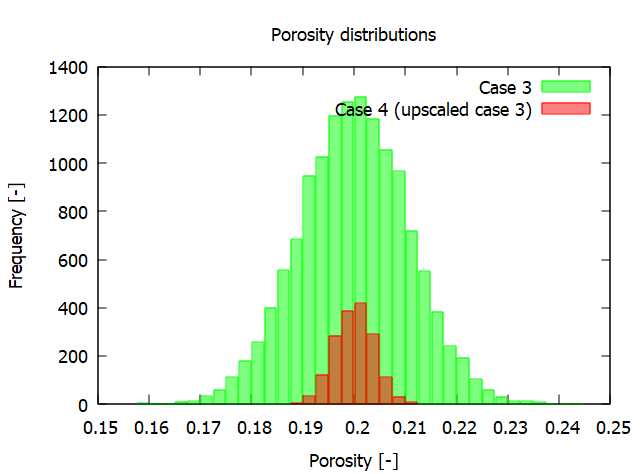
\includegraphics[width=0.82\linewidth]{Images/37}
	\caption{Porosity distribution for case 3 and its upscaled version (case 4).}
	\label{fig:37}
\end{figure}
\begin{figure}[H]
	\centering
	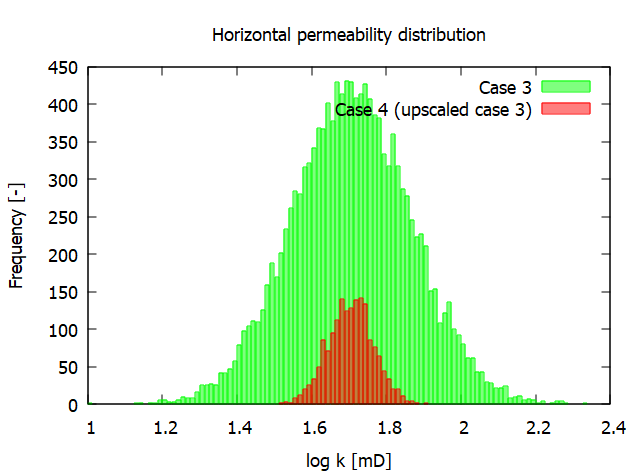
\includegraphics[width=0.82\linewidth]{Images/38}
	\caption{Horizontal permeability distribution for case 3 and its upscaled version (case 4).}
	\label{fig:38}
\end{figure}
\begin{figure}[H]
	\centering
	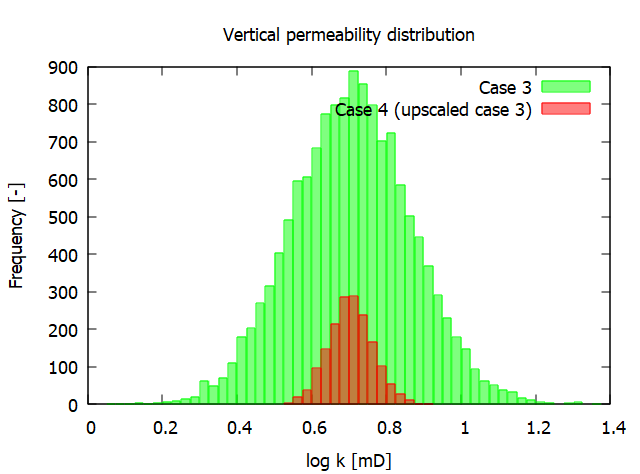
\includegraphics[width=0.82\linewidth]{Images/39}
	\caption{Vertical permeability distribution for case 3 and its upscaled version (case 4).}
	\label{fig:39}
\end{figure}
\begin{figure}[H]
	\centering
	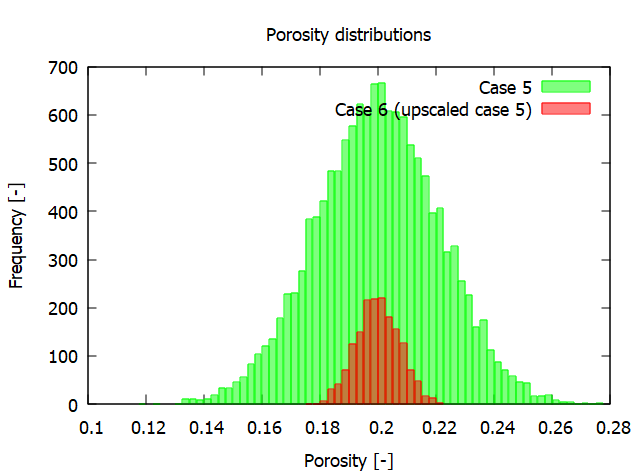
\includegraphics[width=0.82\linewidth]{Images/42}
	\caption{Porosity distribution for case 5 and its upscaled version (case 6).}
	\label{fig:42}
\end{figure}
\begin{figure}[H]
	\centering
	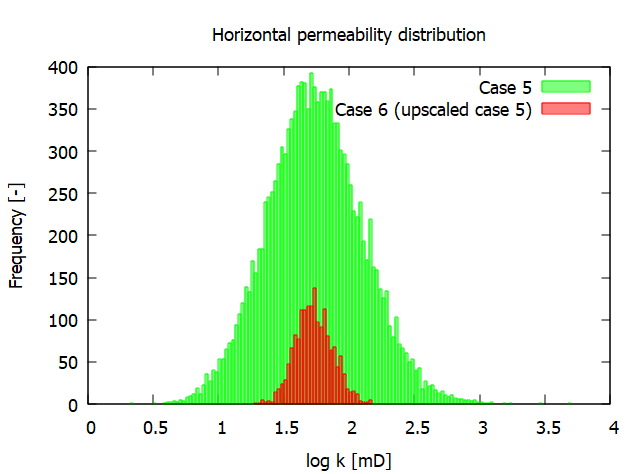
\includegraphics[width=0.82\linewidth]{Images/41}
	\caption{Horizontal permeability distribution for case 5 and its upscaled version (case 6).}
	\label{fig:41}
\end{figure}
\begin{figure}[H]
	\centering
	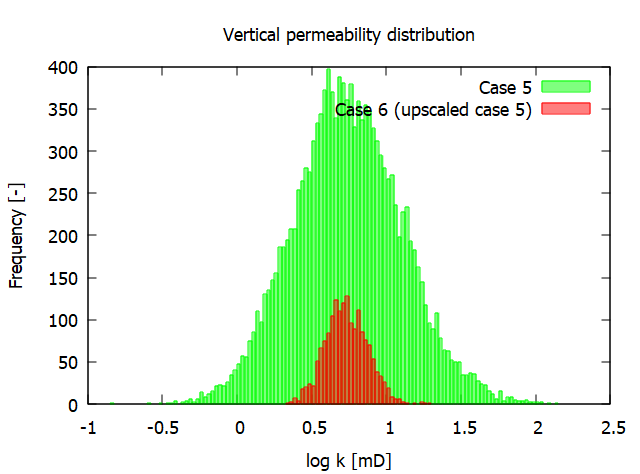
\includegraphics[width=0.82\linewidth]{Images/40}
	\caption{Vertical permeability distribution for case 5 and its upscaled version (case 6).}
	\label{fig:40}
\end{figure}
\begin{figure}[H]
	\centering
	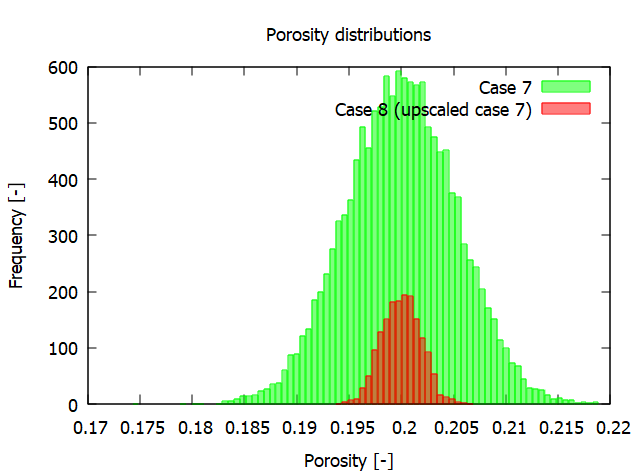
\includegraphics[width=0.82\linewidth]{Images/43}
	\caption{Porosity distribution for case 7 and its upscaled version (case 8).}
	\label{fig:43}
\end{figure}
\begin{figure}[H]
	\centering
	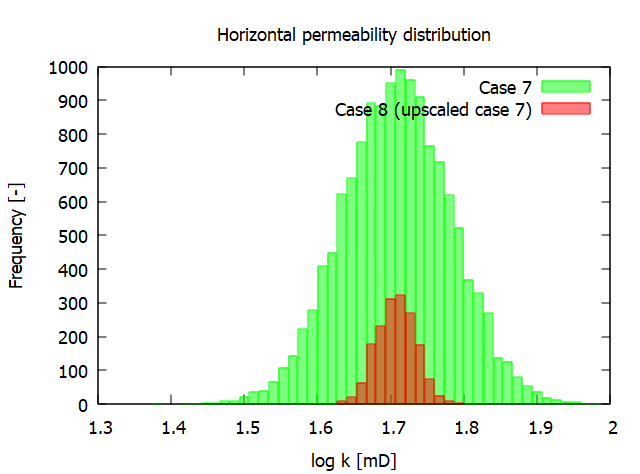
\includegraphics[width=0.82\linewidth]{Images/45}
	\caption{Horizontal permeability distribution for case 7 and its upscaled version (case 8).}
	\label{fig:45}
\end{figure}
\begin{figure}[H]
	\centering
	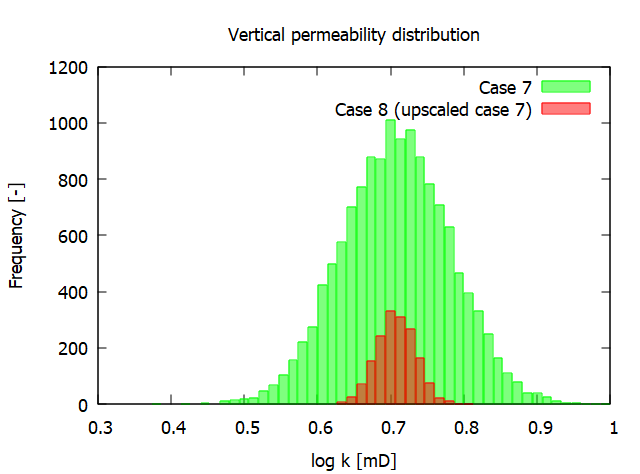
\includegraphics[width=0.82\linewidth]{Images/44}
	\caption{Vertical permeability distribution for case 7 and its upscaled version (case 8).}
	\label{fig:44}
\end{figure}
Looking at Figures \ref{fig:37} to \ref{fig:39} above, one could notice that the red columns (upscaled model) are smaller than the green ones (fine model). This is explained by the fact that the number of grid blocks in the coarse model (upscaled) is eight times inferior to the number of grid blocks in the fine model. Since the vertical axis displays the frequency in absolute terms, the upscaled model should have smaller columns than its fine-grid version. The images above also show that the dispersion in the fine-grid models is higher than in its upscaled counterparts. This decrease in dispersion is a natural characteristic of upscaling since averaging reduces dispersion.